\documentclass{article}
\usepackage{epsfig}
\usepackage{graphicx}
%\usepackage[a4paper, total={6in, 10in}]{geometry}
\usepackage[table]{xcolor}
\usepackage{tikz}
\title{CS345 Programming Assignment 1 \\ }
\author{\vspace{2mm} \large Ayush Agarwal, 13180 \\ M.Arunothia, 13378}
\date{}
\begin{document}
\maketitle
\section{Red-Blue line segments}
\subsection{Algorithmic Description}
For the given $2*n$ line segments ($n$ vertical red and $n$ horizontal blue) (inside the square defined by (0,0) and (1,1))  our implementation does the following to find the number of intersection. \\*
\begin{itemize}
\item We use a line sweep along the Y-direction.
\begin{center}
\begin{tikzpicture}
\draw[step=1cm,gray,very thin] (-2,-2) grid (6,6);
\filldraw[fill=white, draw=black] (-2,-2) rectangle (6,6);
\draw[green,thick,dashed] (-2,0) -- (6,0);
\draw[blue,thick] (0,0) -- (2,0);
\draw[blue,thick] (3,3) -- (5.5,3);
\draw[blue,thick] (1.5,-1.5) -- (4,-1.5);
\draw[blue,thick] (-1.8,2) -- (2,2);
\draw[red,thick] (1,-0.5) -- (1,4);
\draw[red,thick] (-1,3) -- (-1,5.5);
\draw[red,thick] (4,1.7) -- (4,5.8);
\draw[red,thick] (2.7,0) -- (2.7,5);
\node [yellow] at (2.7,0) {\textbullet};
\node [yellow] at (1,-0.5) {\textbullet};
\node [yellow] at (-1,3) {\textbullet};
\node [yellow] at (4,1.7) {\textbullet};
\node [violet] at (2.7,5) {\textbullet};
\node [violet] at (1,4) {\textbullet};
\node [violet] at (-1,5.5) {\textbullet};
\node [violet] at (4,5.8) {\textbullet};
\node [violet] at (2.7,5) {\textbullet};
\end{tikzpicture}
\end{center}
\item The green dashed line in the above figure shows our sweep line. This basically means that the horizontal blue lines are processed in increasing $y$ co-ordinates.
\item All yellow points (bottom point of red lines) that lies below or on the sweep line indicate those red lines that can potentially cause an intersection with the blue line. So, the $x$-coordinates of these yellow points are inserted into the BST maintained.
\item All violet points (top point of red lines) that lies below the sweep line indicate those red lines that can no longer cause an intersection with the blue line. So, the $x$-coordinates of these violet points are deleted from the BST maintained.
\item Now the number of intersections of this blue line (say is defined by $(x_1,y),(x_2,y)$)  are found by finding the number of nodes in the BST having $x$ in the range $[x_1,x_2]$.
\item To optimize the above implementation, the BST was augmented by sub-tree size along with usual node data.
\item Two implementations of the range count was done, with first one being submitted -
\begin{itemize}
\item By finding count of $x > x_2$ and $x >= x_1$ and by taking their difference for the required range. 
\item by LCA method
\end{itemize} 
\end{itemize}
\subsection{Implementation Description}
\begin{itemize}
\item {\bf Language of Implementation} - C++ 
\item {\bf Number of lines of Code} - 190 lines (including time and random generator functions)\\*
\item {\bf Configuration of System used for Experiment}
\begin{center}
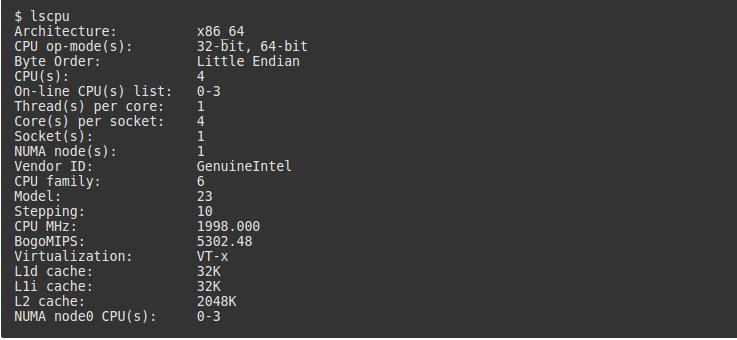
\includegraphics[scale=0.5]{system_conf.png}
\end{center}
\item {\bf Number of repetitions} made for a given {\bf $n$} is {\bf $10^7/n$}. 
\item {\bf Range of $n$ } is {\bf $\{1,10,10^2, 10^3, 10^4, 10^5, 10^6, 10^7 \} $}
\end{itemize}
\hspace*{-2.5cm}\begin{tabular}{|p{1cm}|p{2.5cm}|p{2.5cm}|p{2cm}|p{2cm}|p{4cm}|}
 \hline
 \multicolumn{6}{|c|}{Result Table} \\
 \hline
 $n$   & Time(seconds) & No. of Intersections & $n^2/9$ &  $n *\log n $ & $(10^7 * Time/n* \log n)$\\
 \hline 
 $1$   	& $0$ 		& $0.1111$	& $ 0.11 $ 		& $ 0 $  		& $ -- $	\\
 \hline
 $10$  	& $4.00 * 10^{-6}$	& $11.1052$ & $ 11.11 $		& $ 33.2 $		& $ 1.20 $	\\
 \hline
 $10^2$	& $7.00 * 10^{-5}$	& $1110.92$	& $ 1111.11$		& $ 664 $		& $ 1.05 $	\\
 \hline
 $10^3$	& $0.0011$	& $111082$	& $ 111111.11 $ 	& $	9960	 $		& $ 1.10 $	\\
 \hline
 $10^4$	& $0.015$  	& $1.11* 10^7 $	& $ 1.11 * 10^7  $	& $	132800 $		& $ 1.13 $\\
 \hline
 $10^5$	& $0.25$ 	& $1.11* 10^9$& $ 1.11 * 10^7	$ 	& $	1.66 * 10^6$	& $ 1.50 $	\\
 \hline
 $10^6$	& $4.8$		& $1.11* 10^{11}$& $ 1.11 * 10^7 $	& $	1.992 * 10^7$	& $ 2.41 $	\\
 \hline
 $10^7$	& $62$		& $1.11* 10^{13}$& $ 1.11 * 10^7 $	& $	2.324 * 10^8$	& $ 2.67 $	\\
 \hline
\end{tabular}

\subsection{Plot}

\subsection{Inferences}
\begin{itemize}
\item From Result Table, we can see that execution time of the algorithm is $O(n*logn)$
\item From $n=10^2$ to $n=10^7$ we can notice a steady increase in the $Time/(n*log n)$ ratio. 
\item From Result Table, we can see that on an average, the number of intersections of the red-blue line segments when generated uniformly randomly in $(0,1)$ is $n^2/2$
\subsubsection{Bonus Question Proof}
From our uniform generation we have that ($0<=x_1<=1$), ($0<=x_2<=1$), ($0<=y_1<=1$), ($0<=y_2<=1$), ($0<=x<=1$) and ($0<=y<=1$) are random variables with probability distribution function as $1$ in $[0,1]$ and 0 otherwise. Therefore, the probability of $x$ lying between $[x_1,x_2]$ will be (taking $x_1<=x_2$) -
\begin{center}
$\int_{0}^{1} {$\int_{x_1}^{1} {$\int_{x}^{1} 1 * dx_2 $} * dx * $} dx_1$
= 1/6
\end{center}
Similarly for $x_1>=x_2$ it will be $1/6$. Implying overall probability of $x$ lying between $x_1$ and $x_2$ is $1/3$. \\*
Blue and Red line segments will intersect when 
\begin{center}
$x$ lies between $x_1$ and $x_2$ \\*
and \\*
$y$ lies between $y_1$ and $y_2$ \\*
\end{center}
Implies probability of one blue and one red line segment intersection is -
\begin{center}
= $1/3 * 1/3 = 1/9$ \\*
As $x$ and $y$ are independent random variables here.
\end{center}
There are $n^2$ pairs of $(red,blue)$ line segments. Implying on an average when $n$ is pretty large, the number of intersections should be
\begin{center}
 = $n^2 * 1/9$ \\*
 = $n^2/9$
\end{center} 
\item  We tried random generation also based on the constraints - 
\begin{itemize}
\item $0<=x_2<=1$, $0<=x_1<=x_2$ and $0<=x<=1$
\item $0<=y_2<=1$, $0<=y_1<=x_2$ and $0<=y<=1$
\end{itemize}
In this case we got average number of intersections = $n^2/16$, which can again be proved like above and is also very intuitive.
\begin{center}
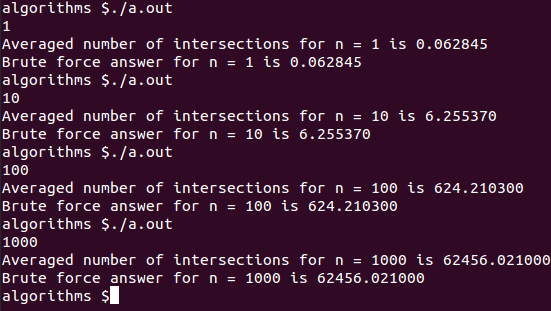
\includegraphics[scale=0.5]{out.png}
\end{center}
\item If you notice the output shown above, the answer is matching exactly with the brute force answer, indicating the code should be right. But, this code does NOT work properly with the corner case of overlapping verticals and it got a WA on judge. This should be because, when double/float values are randomly generated it is very unlikely that they end up being same!!
\item Though we are NOT balancing the BST after any insertion, this implementation shows that running time is indeed in $O(n*log(n))$, showing the power of a randomized input. 
\end{itemize}
\end{document}
